\paragraph{Escalera de modelos.}
La tabla~\ref{tab:deepresults} resume los modelos anclados a BirdNET y la tabla~\ref{tab:deepm3} detalla la exhaustividad por nivel de atenuación.
Con 0,25 como umbral, BirdNET detecta el \deepAttBirdnetSix\,\% de los cantos validados cuando se atenúan 6\,dB y el \deepAttBirdnetTwelve\,\% a 12\,dB.
La media de los cuatro niveles es $S = \deepAttBirdnet$\,\%. Esa caída tan rápida es en parte un efecto de selección: todo canto validado
superó 0,25 en su ventana original, y muchos lo hicieron por poco.

\begin{table}[H]
  \centering\small
  \caption{Modelos anclados a BirdNET, con predicciones fuera de muestra. M1 es el control de seguridad (D1: el intervalo de $\Delta$ no baja de $-0{,}01$).
  En M3, \emph{original} es la fracción de cantos validados sin atenuar que el modelo sigue marcando con el mismo volumen de alertas, y $S$ es la media
  de los niveles de 6 a 24\,dB (D3: el intervalo de $\Delta S$ queda por encima de cero).}\label{tab:deepresults}
  \fittab{tab_deep_results.tex}
\end{table}

\begin{table}[H]
  \centering\small
  \caption{Exhaustividad (\%) sobre cantos validados, por nivel de atenuación, con el mismo volumen de alertas que BirdNET. Última columna:
  media de los niveles atenuados con un 1\,\% de falsas alarmas sobre ventanas donde BirdNET calla.}\label{tab:deepm3}
  \fittab{tab_deep_m3.tex}
\end{table}

\paragraph{Qué ganan las correcciones y qué cuestan.}
Las correcciones libres mejoran la detección de cantos atenuados, pero poco. La MLP sube $S$ de \deepAttBirdnet{} a \deepAttMlp\,\%: \deepAttDeltaMlp{} puntos,
con un intervalo de \deepAttCiMlp. La ganancia es estadísticamente detectable en los cuatro escalones (D3) y va de \deepAttDeltaLinear{} a \deepAttDeltaDeep{}
puntos. El precio es alto. La mAP limpia cambia en \deepCleanDeltaMlp{} (IC \deepCleanCiMlp) y ninguna corrección libre
pasa el control de seguridad. Además, con el mismo volumen de alertas la MLP solo conserva el \deepAttMlpZero\,\% de las detecciones validadas
(columna \emph{original}).

La causa está en lo que estas etiquetas permiten aprender. Todos los positivos sin atenuar superan 0,25. Las mezclas atenuadas, que también son
positivos, caen en buena parte en la zona gris, donde BirdNET puntúa entre 0,05 y 0,25. En esa zona no hay ningún negativo etiquetado.
El modelo aprende entonces a subir la puntuación de toda la zona gris, no a distinguir dentro de ella. Con el umbral de 0,25, la MLP propone el
\deepGrayUpMlp\,\% de los pares de la zona gris y \deepSilentUpMlp{} pares donde BirdNET callaba, y solo deja de proponer \deepValidLostMlp{} de las
\deepCatP{} validadas. Los datos no dicen si esas propuestas nuevas son cantos reales que BirdNET no vio o falsas alarmas. Al igualar el volumen de
alertas, desplazan a detecciones validadas, y por eso la exhaustividad sobre los cantos débiles apenas cambia.

La pérdida de mAP limpia se concentra en especies con pocos positivos, donde basta que unas pocas ventanas sin canto conocido superen a las
validadas. Calculada dentro de cada pliegue, la mAP limpia de la MLP es \deepCleanFoldMlp{} frente a \deepCleanFoldBirdnet{} de BirdNET. La medida conjunta
la deja en \deepCleanMlp, y es la que cuenta, porque el modelo se usaría sobre todas las grabaciones a la vez. Esa diferencia explica que la
selección anidada, que mide dentro de un pliegue, no anticipara la pérdida. También explica que los intervalos de la mAP limpia sean asimétricos:
la pérdida depende de pocas sesiones, y en las réplicas de bootstrap donde esas sesiones no entran casi desaparece.

\paragraph{La profundidad no aporta.}
Afinar \code{POST_CONV} da $S = \deepAttPost$\,\% y añadir los sub-bloques 4-3 y 4-4 da \deepAttDeep\,\%. Ninguna diferencia entre escalones se separa del
cero (tabla~\ref{tab:deepladder}): una corrección del \emph{embedding} consigue lo mismo que mover las capas convolucionales.
Como el escalón de los sub-bloques no mejora al de \code{POST_CONV}, el del bloque 4 completo no se entrenó, según la regla fijada de antemano.
La selección anidada mantuvo los pesos cerca de BirdNET (tabla~\ref{tab:deepgrid}).

\begin{table}[H]
  \centering\small
  \caption{Comparaciones pareadas entre modelos (mismos pliegues, misma semilla y mismo banco de mezclas).}\label{tab:deepladder}
  \fittab{tab_deep_ladder.tex}
\end{table}

\begin{table}[H]
  \centering\small
  \caption{Configuración que eligió cada pliegue con su pliegue interno y deriva relativa media de los pesos convolucionales respecto de BirdNET.
  En las cabezas, d$N$ indica un decaimiento $N$ de la capa de salida (cuanto mayor, más cerca de BirdNET) y el signo + un peso mayor de la destilación.
  En las capas convolucionales la rejilla va de \emph{muy prudente} a \emph{libre}. $^{*}$: ninguna configuración cumplía el control en el pliegue
  interno y se tomó la de mayor mAP limpia.}\label{tab:deepgrid}
  \fittab{tab_deep_grid.tex}
\end{table}

\paragraph{Ablaciones.}
Las ablaciones reutilizan la configuración que eligió cada pliegue para la MLP.
\begin{itemize}
  \item \textbf{Sin mezclas atenuadas} la ganancia desaparece ($S = \deepAttMlpNoMix$\,\%). Lo poco que se gana viene de enseñar al modelo cantos más débiles.
  \item \textbf{Con etiquetas estrictas}, es decir, tratando como negativo todo lo no validado, el índice de fuga sube de \deepSliMlp{} a \deepSliMlpStrict.
        El modelo aprende a distinguir lo revisado de lo no revisado, que es lo que el protocolo quería evitar.
  \item \textbf{Con otra semilla} se obtiene $S = \deepAttMlpSeed$\,\%. La diferencia entre semillas (0,2 puntos) es menor que la ganancia.
  \item \textbf{Con negativos certificados.} Cuando una especie calla en los dos ingredientes de una mezcla y BirdNET la puntúa por encima de 0,05,
        esa puntuación es una falsa alarma segura. Hay \deepMixNegatives{} pares así en las mezclas de entrenamiento, y son los únicos negativos disponibles
        en la zona gris. Usarlos no cambia el resultado ($S = \deepAttMlpNeg$\,\%, mAP limpia \deepCleanMlpNeg): son demasiado pocos.
\end{itemize}

\paragraph{Corrección acotada.}
Tras ver que las cabezas no pasaban el control se añadió una variante que no estaba prevista: recortar la corrección aprendida a $\pm 0{,}9$ logits.
Con ese límite, un par donde BirdNET calla no puede superar a uno validado. El control de seguridad se cumple entonces por construcción, de modo que
D1 no cuenta como evidencia a favor de esta variante. La variante conserva casi todas las detecciones validadas (\deepAttMlpBZero\,\% con la MLP), pero la
ganancia en cantos atenuados desaparece (\deepAttDeltaMlpB{} puntos). La ganancia de la corrección libre procedía, por tanto, de correcciones grandes
sobre ventanas que BirdNET puntúa muy bajo. La figura~\ref{fig:deeptradeoff} resume ambas familias y la figura~\ref{fig:deepm3} muestra el cambio por
nivel de atenuación.

\begin{figure}[H]
  \centering
  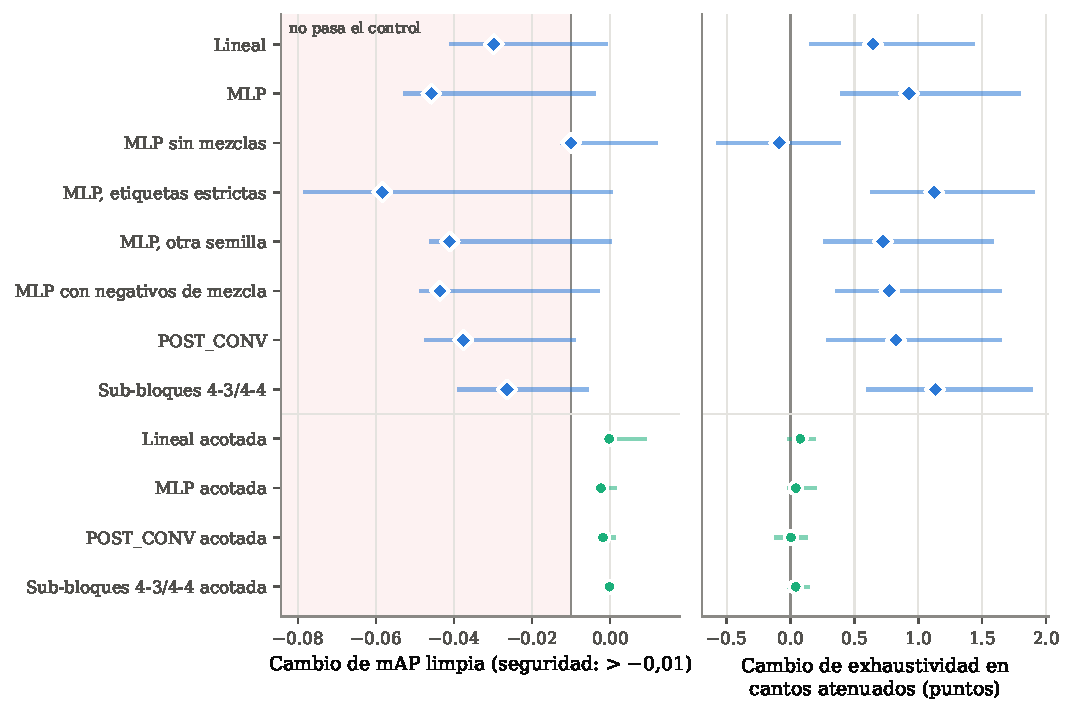
\includegraphics[width=0.92\linewidth]{fig_deep_tradeoff.pdf}
  \caption{Cambio respecto de BirdNET de cada modelo anclado, con intervalos del 95\,\%. Izquierda: mAP limpia; a la izquierda de la línea de $-0{,}01$
  no se pasa el control de seguridad. Derecha: exhaustividad media sobre cantos atenuados con el mismo volumen de alertas. Rombos: corrección libre.
  Círculos: corrección acotada.}\label{fig:deeptradeoff}
\end{figure}

\begin{figure}[H]
  \centering
  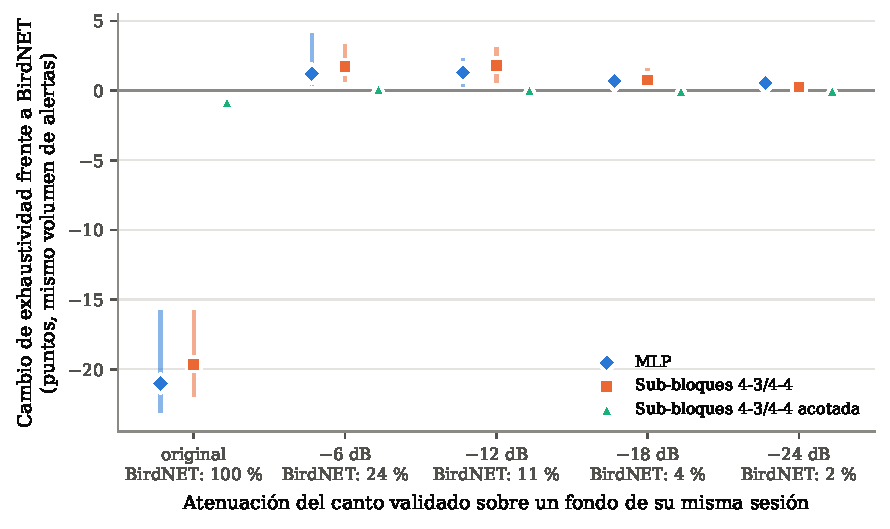
\includegraphics[width=0.88\linewidth]{fig_deep_m3.pdf}
  \caption{Cambio de exhaustividad respecto de BirdNET en cada nivel de atenuación, con el mismo volumen de alertas e intervalos del 95\,\%.
  Bajo cada nivel se indica la exhaustividad de BirdNET.}\label{fig:deepm3}
\end{figure}

\paragraph{Rechazos expertos: verificación en dos etapas.}
El segundo problema medible es descartar falsos positivos entre las propuestas de BirdNET. BirdNET deja por encima de cada rechazo, de media, el
\deepRejPctBirdnet\,\% de las detecciones validadas de su especie y grabadora (M2 = \deepRejBirdnet). Las sondas entrenadas desde cero quedan muy por
debajo de BirdNET como detectores independientes (mAP limpia \deepCleanProbeNew). En cambio, ordenan las propuestas de BirdNET mejor que él:
M2 = \deepRejProbeNew, una diferencia de \deepRejDeltaProbeNew{} con un intervalo de \deepRejCiProbeNew{} (tabla~\ref{tab:deepverifiers} y
figura~\ref{fig:deepm2}).

El esquema de dos etapas aprovecha las dos cosas: BirdNET decide qué se propone y la sonda ordena las propuestas. El conjunto de alertas es
exactamente el de BirdNET, de modo que la exhaustividad no cambia. Pasa el control de seguridad (\deepCleanDeltaTwoStage, IC \deepCleanCiTwoStage) y
mejora M2 en \deepRejDeltaTwoStage. Con un corte que conserva el 95\,\% de las detecciones validadas de cada especie, la sonda deja por debajo
\deepRejRemovedTwoStage{} de los \deepRejections{} rechazos. Con la puntuación de BirdNET serían \deepRejRemovedBirdnet. Un verificador de cinco variables
derivadas de BirdNET (su puntuación, el margen sobre la clase competidora, el contexto de la grabación) no mejora M2
(\deepRejDeltaVerifier, IC \deepRejCiVerifier): lo que separa un rechazo de una validada no está en la salida de BirdNET, sino en el \emph{embedding}.

\begin{table}[H]
  \centering\small
  \caption{Colocación de los rechazos expertos (M2) y rechazos que quedan por debajo del corte que conserva el 95\,\% de las validadas de su especie.
  D1 y D2 son las reglas de la sección~\ref{sec:protocolo}.}\label{tab:deepverifiers}
  \fittab{tab_deep_verifiers.tex}
\end{table}

\begin{figure}[H]
  \centering
  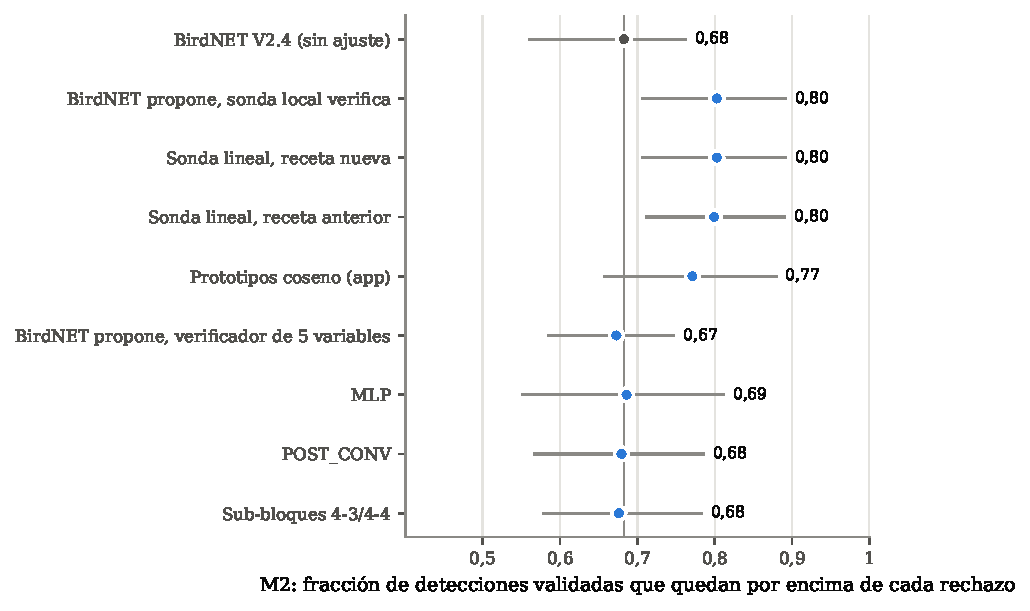
\includegraphics[width=0.88\linewidth]{fig_deep_m2.pdf}
  \caption{M2 por modelo con intervalos del 95\,\%. La línea vertical oscura marca el valor de BirdNET; 0,5 equivale a ordenar al azar.}\label{fig:deepm2}
\end{figure}

Tres cautelas. Solo hay \deepRejections{} rechazos, concentrados en pocas sesiones, y los intervalos son anchos. La mejora se mide entre sesiones
de las mismas seis grabadoras: no dice cómo se comportaría la sonda en un sitio nuevo. Y M2 compara puntuaciones de los cinco modelos de la validación
cruzada, que no están calibrados entre sí; ese ruido añadido tiende a perjudicar a la sonda, pero no se ha medido.

\paragraph{Decisión.}
Según las reglas fijadas de antemano, el esquema de dos etapas es exportable: cumple D1 y D2 sin pérdida en la exhaustividad. Las correcciones
libres cumplen D3 con una ganancia pequeña, pero no D1: no son exportables. Las acotadas cumplen D1 por construcción y no mejoran M3. Entre ellas,
la corrección lineal acotada también mejora M2 (\deepRejDeltaLinearB, IC \deepRejCiLinearB), menos de la mitad que las dos etapas, que además son más
simples. Se exporta, por tanto, el esquema de dos etapas.

\subsection{Integración del verificador}\label{sec:verificador}
La aplicación carga el verificador si encuentra el archivo \code{verificador_local.npz} junto al clasificador local. No cambia qué se detecta:
BirdNET, con la lista local y los umbrales por especie, sigue decidiendo las detecciones. El verificador añade a cada una la puntuación de la sonda y
marca como \emph{CONDESAN · revisar} las que quedan por debajo del percentil 5 de las detecciones validadas de su especie. Las especies con menos de
20 validadas no se marcan. Medido con predicciones fuera de muestra, marca el \deepFlagValid\,\% de las detecciones validadas, \deepFlagRejected{} de los
\deepFlagRejectedOf{} rechazos expertos y el \deepFlagUnreviewed\,\% de las propuestas sin revisar. Los cortes proceden de esas predicciones fuera de muestra,
mientras que la sonda que se distribuye se ajusta con todas las sesiones. En las sesiones que no intervinieron en el ajuste de sus pesos, esa sonda
marca el \deepFlagHeldValid\,\% de las validadas (\deepFlagHeldMarked{} de \deepFlagHeldOf), algo distinto del 5\,\% nominal: la marca es una ayuda para
priorizar la escucha, no un filtro. El archivo contiene los pesos de la sonda, no los de BirdNET, y no se publica en el repositorio.

\subsection{Lectura de los resultados y límites}\label{sec:lectura2}
\begin{enumerate}
  \item \textbf{El límite está en las etiquetas, no en el modelo.} Se afinaron las capas profundas de BirdNET con una pérdida adaptada al proceso de
        revisión, y la profundidad no aportó nada medible. Con estas etiquetas no se puede enseñar ni demostrar que un modelo detecta más que BirdNET, porque
        todo lo que se sabe está por encima de 0,25.
  \item \textbf{Lo que desbloquea la mejora es anotar la zona gris.} Hacen falta ventanas con puntuación de BirdNET entre 0,05 y 0,25 escuchadas por un
        experto, con presencias y ausencias. La muestra aleatoria de 300 ventanas ya preparada y la lista de ventanas en discrepancia de esta fase
        apuntan justo ahí (sección~\ref{sec:ayuda}).
  \item \textbf{La mejora validada es descartar falsos positivos}, no detectar más. Es modesta en términos absolutos, porque los expertos rechazaron pocas
        detecciones, pero es la única que estos datos permiten medir sin sesgo.
  \item \textbf{La prueba de cantos atenuados es sintética.} Atenuar un canto y sumarle un fondo no reproduce la reverberación ni el filtrado de un ave
        lejana. Sirve para comparar modelos entre sí, no para estimar cuántos cantos reales se pierden.
  \item \textbf{Cambios respecto del plan inicial.} Los dos primeros se decidieron antes de evaluar los pliegues de prueba del modelo afectado.
        (a) Se añadió una rejilla de regiones de confianza para las cabezas, porque la configuración inicial no cumplía el control en ningún pliegue interno.
        (b) La rejilla de las capas convolucionales se amplió de tres a cinco configuraciones porque los pliegues internos elegían la más agresiva, y las
        filas del clasificador pasaron a seguir la misma región de confianza. Las predicciones de la primera pasada se descartaron sin evaluarse. Aun así,
        los pliegues internos recorren entre todos el conjunto entero, de modo que esta decisión no es del todo independiente de los pliegues de prueba
        y puede favorecer ligeramente a los escalones convolucionales.
        (c) La corrección acotada y la ablación con negativos certificados se añadieron después de ver los resultados de las cabezas, y se presentan
        como análisis posteriores.
        (d) Una revisión independiente del código, hecha con los resultados ya a la vista, encontró dos defectos en el cálculo de M3. En las réplicas de
        bootstrap, una ventana de una sesión no remuestreada podía fijar el umbral; y el umbral se elegía de modo que el modelo nunca superara el volumen
        de alertas de BirdNET, lo que le dejaba algo menos (un 2\,\% de media en el escalón de los sub-bloques). Se corrigieron ambos: ahora el
        volumen se iguala exactamente. Los valores de $S$ cambiaron menos de 0,05 puntos, pero los intervalos se estrecharon, y D3 pasó de \emph{no} a
        \emph{sí} para la corrección lineal y para \code{POST_CONV}, cuyos intervalos antes rozaban el cero ($[-0{,}1;\ +1{,}3]$ y $[-0{,}0;\ +1{,}6]$ puntos).
        Ninguna decisión cambia. La selección anidada se hizo con el cálculo anterior y no se repitió. La misma revisión no encontró fugas de
        información entre pliegues en el entrenamiento.
\end{enumerate}
